\chapter{Wyniki eksperymentów}

Rozdział ten przedstawia wybrane wyniki eksperymentów. Analiza skupia się na podstawowych metrykach opisujących
wydajność algorytmu aktywnego uczenia, czyli liczbie poszczególnych zapytań kierowanych do nauczyciela.
Przedstawiono również, w jaki sposób struktura automatu wpływa na liczbę potrzebnych zapytań
oraz jak wykorzystanie systemu SRS wpływa na proces uczenia.

\section{Podstawowe metryki}

Przedstawione poniżej wykresy zostały wygenerowane na podstawie danych ze scenariuszy benchmarkowych, z użyciem losowego generatora.
Mają na celu wizualizację liczby potrzebnych zapytań dla losowych automatów różniących się liczbą stanów,
rozmiarem alfabetu, jak i alfabetu stosowego.

Poniżej przedstawiona jest początkowa konfiguracja losowego generatora dla wszystkich scenariuszy w tej sekcji:
\begin{verbatim}
NumOfStates = 2
NumOfCalls = 3
NumOfLocals = 3
NumOfReturns = 3
NumOfStackSymbols = 5
density = 0.8
acceptingStatesDensity = 0.3
\end{verbatim}

Każdy ze scenariuszy modyfikował początkową konfigurację generatora poprzez zwiększanie liczby stanów oraz
liczby symboli wybranego typu. Dla każdej konfiguracji zostało wygenerowane 200 automatów,
dla których poszczególne wyniki zostały zebrane i uśrednione w celu pokazania trendów.

\begin{figure}[ht]
    \centering

    \begin{minipage}{0.85\textwidth}
        \centering

        \begin{minipage}{0.48\textwidth}
            \centering
            \begin{tikzpicture}
    \begin{axis}[
        baseMetricsHeatmap,
        colorbar = true,
        point meta min=0,
        point meta max=200000,
        xlabel={liczba symboli call},
    ]
    \addplot [
        matrix plot*,
        point meta=explicit,
        mesh/rows=7,
    ] coordinates {
        (3, 2) [925.745]
        (3, 4) [6152.28]
        (3, 6) [16820.8]
        (3, 8) [32521.3]
        (3, 10) [56390.4]
        (3, 12) [83094.1]
        (3, 14) [118000]
        (3, 16) [163348]
        (5, 2) [1064.88]
        (5, 4) [7052.32]
        (5, 6) [19791.7]
        (5, 8) [38043.8]
        (5, 10) [64132.3]
        (5, 12) [101389]
        (5, 14) [140461]
        (5, 16) [186509]
        (7, 2) [1173.72]
        (7, 4) [7909.88]
        (7, 6) [20961.3]
        (7, 8) [41537.2]
        (7, 10) [69185.2]
        (7, 12) [109299]
        (7, 14) [152927]
        (7, 16) [208644]
        (9, 2) [1268.79]
        (9, 4) [8534.83]
        (9, 6) [23123]
        (9, 8) [47404]
        (9, 10) [76616.3]
        (9, 12) [119156]
        (9, 14) [169757]
        (9, 16) [223338]
        (11, 2) [1328.44]
        (11, 4) [9433.5]
        (11, 6) [24736.3]
        (11, 8) [50014]
        (11, 10) [83825.5]
        (11, 12) [129716]
        (11, 14) [177398]
        (11, 16) [248165]
        (13, 2) [1408.52]
        (13, 4) [10166.1]
        (13, 6) [26009.7]
        (13, 8) [54584.3]
        (13, 10) [89500.1]
        (13, 12) [139050]
        (13, 14) [190277]
        (13, 16) [259680]
        (15, 2) [1497.38]
        (15, 4) [10800.6]
        (15, 6) [29926.6]
        (15, 8) [58864.3]
        (15, 10) [92320.5]
        (15, 12) [141288]
        (15, 14) [207244]
        (15, 16) [283816]
    };
    \end{axis}
    \end{tikzpicture}
        \end{minipage}
        \hfill
        \begin{minipage}{0.48\textwidth}
            \centering
            \begin{tikzpicture}
    \begin{axis}[
        baseMetricsHeatmap,
        colorbar = false,
        point meta min=0,
        point meta max=200000,
        xlabel={liczba symboli return},
    ]
    \addplot [
        matrix plot*,
        point meta=explicit,
        mesh/rows=7,
    ] coordinates {
        (3, 2) [925.745]
        (3, 4) [6152.28]
        (3, 6) [16820.8]
        (3, 8) [32521.3]
        (3, 10) [56390.4]
        (3, 12) [83094.1]
        (3, 14) [118000]
        (3, 16) [163348]

        (5, 2) [1487.34]
        (5, 4) [9509.58]
        (5, 6) [26328.9]
        (5, 8) [50495.5]
        (5, 10) [87853.7]
        (5, 12) [128784]
        (5, 14) [182956]
        (5, 16) [250333]

        (7, 2) [2049.76]
        (7, 4) [13652.1]
        (7, 6) [37144]
        (7, 8) [71036.4]
        (7, 10) [118153]
        (7, 12) [177753]
        (7, 14) [243029]
        (7, 16) [325197]

        (9, 2) [2513.58]
        (9, 4) [17344.4]
        (9, 6) [45553.8]
        (9, 8) [89955.9]
        (9, 10) [147382]
        (9, 12) [221523]
        (9, 14) [315642]
        (9, 16) [414558]

        (11, 2) [3087.79]
        (11, 4) [20546.2]
        (11, 6) [56681.7]
        (11, 8) [113060]
        (11, 10) [183767]
        (11, 12) [270795]
        (11, 14) [381161]
        (11, 16) [497551]

        (13, 2) [3646.57]
        (13, 4) [24036.9]
        (13, 6) [66560.6]
        (13, 8) [129589]
        (13, 10) [221977]
        (13, 12) [336061]
        (13, 14) [474632]
        (13, 16) [610764]
        
        (15, 2) [4135.26]
        (15, 4) [27505.4]
        (15, 6) [74951.5]
        (15, 8) [153354]
        (15, 10) [261704]
        (15, 12) [383806]
        (15, 14) [527092]
        (15, 16) [705174]
    };
    \end{axis}
    \end{tikzpicture}
        \end{minipage}

        \vspace{0.5em}

        \begin{minipage}{0.48\textwidth}
            \centering
            \begin{tikzpicture}
    \begin{axis}[
        baseMetricsHeatmap,
        colorbar = false,
        point meta min=0,
        point meta max=200000,
        xlabel={liczba symboli local},
    ]
    \addplot [
        matrix plot*,
        point meta=explicit,
        mesh/rows=7,
    ] coordinates {
        (3, 2) [925.745]
        (3, 4) [6152.28]
        (3, 6) [16820.8]
        (3, 8) [32521.3]
        (3, 10) [56390.4]
        (3, 12) [83094.1]
        (3, 14) [118000]
        (3, 16) [163348]

        (5, 2) [982.92]
        (5, 4) [6856.96]
        (5, 6) [19249.9]
        (5, 8) [38075.8]
        (5, 10) [63621.8]
        (5, 12) [96444.5]
        (5, 14) [136082]
        (5, 16) [182040]

        (7, 2) [1051.5]
        (7, 4) [7331.17]
        (7, 6) [20551.9]
        (7, 8) [41332.1]
        (7, 10) [69035.4]
        (7, 12) [104971]
        (7, 14) [152581]
        (7, 16) [204913]

        (9, 2) [1185.05]
        (9, 4) [7878.74]
        (9, 6) [21467.2]
        (9, 8) [43273.4]
        (9, 10) [76816.3]
        (9, 12) [116772]
        (9, 14) [165006]
        (9, 16) [225452]

        (11, 2) [1191.87]
        (11, 4) [8172.77]
        (11, 6) [23787.1]
        (11, 8) [46539.8]
        (11, 10) [80194.5]
        (11, 12) [127723]
        (11, 14) [181584]
        (11, 16) [242747]

        (13, 2) [1253.86]
        (13, 4) [8801.72]
        (13, 6) [24263.4]
        (13, 8) [51984.1]
        (13, 10) [90632]
        (13, 12) [138839]
        (13, 14) [193101]
        (13, 16) [267909]

        (15, 2) [1357.53]
        (15, 4) [9456.6]
        (15, 6) [26841.2]
        (15, 8) [54986.9]
        (15, 10) [94727.2]
        (15, 12) [142968]
        (15, 14) [213350]
        (15, 16) [286288]
    };
    \end{axis}
    \end{tikzpicture}
        \end{minipage}
        \hfill
        \begin{minipage}{0.48\textwidth}
            \centering
            \begin{tikzpicture}
    \begin{axis}[
        baseMetricsHeatmap,
        colorbar = false,
        point meta min=0,
        point meta max=200000,
        xlabel={liczba symboli stosowych},
        xmin=5,
    ]
    \addplot [
        matrix plot*,
        point meta=explicit,
        mesh/rows=6,
    ] coordinates {
        (5, 2) [693.69]
        (5, 4) [3630.69]
        (5, 6) [10014.1]
        (5, 8) [18955.7]
        (5, 10) [31231.3]
        (5, 12) [47282.3]
        (5, 14) [69600.3]
        (5, 16) [97164.3]

        (7, 2) [943.2]
        (7, 4) [4911.38]
        (7, 6) [12337.7]
        (7, 8) [25055.8]
        (7, 10) [40731.3]
        (7, 12) [63010.6]
        (7, 14) [90310.8]
        (7, 16) [123967]

        (9, 2) [1090.38]
        (9, 4) [5805.6]
        (9, 6) [14962.8]
        (9, 8) [30048.8]
        (9, 10) [48059.3]
        (9, 12) [76431.9]
        (9, 14) [109298]
        (9, 16) [141495]

        (11, 2) [1392.17]
        (11, 4) [6979.9]
        (11, 6) [17620.7]
        (11, 8) [36787.5]
        (11, 10) [60501]
        (11, 12) [88381.8]
        (11, 14) [130361]
        (11, 16) [177646]

        (13, 2) [1524.96]
        (13, 4) [7955.12]
        (13, 6) [21508.1]
        (13, 8) [40779.4]
        (13, 10) [67889.5]
        (13, 12) [104478]
        (13, 14) [153326]
        (13, 16) [208076]

        (15, 2) [1731.02]
        (15, 4) [9522.93]
        (15, 6) [23218.6]
        (15, 8) [45745.6]
        (15, 10) [81083.5]
        (15, 12) [117392]
        (15, 14) [165269]
        (15, 16) [238512]
    };
    \end{axis}
    \end{tikzpicture}
        \end{minipage}
    \end{minipage}
    \hfill
    \begin{minipage}{0.08\textwidth}
    \centering
    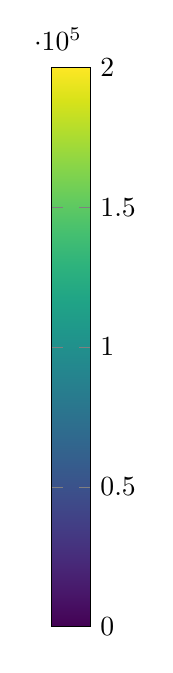
\begin{tikzpicture}
    \begin{axis}[
        hide axis,
        scale only axis,
        height=8.8cm,
        width=0pt,
        point meta min=0,
        point meta max=200000,
        colormap name=viridis,
        colorbar = true,
        colorbar style={
            height=7.1cm,
        }
    ]
    \addplot [draw=none] coordinates {(0,0)};
    \end{axis}
    \end{tikzpicture}
    \end{minipage}

    \caption{Średnia liczba zapytań typu membership query}
\end{figure}

\begin{figure}[ht]
    \centering

    \begin{minipage}{0.85\textwidth}
        \centering

        \begin{minipage}{0.48\textwidth}
            \centering
            \begin{tikzpicture}
    \begin{axis}[
        baseMetricsHeatmap,
        colorbar = true,
        point meta min=0,
        point meta max=200000,
        xlabel={liczba symboli call},
    ]
    \addplot [
        matrix plot*,
        point meta=explicit,
        mesh/rows=7,
    ] coordinates {
        (3, 2) [682.48]
        (3, 4) [4818.62]
        (3, 6) [13329.6]
        (3, 8) [25892]
        (3, 10) [44815.9]
        (3, 12) [66036.6]
        (3, 14) [93586]
        (3, 16) [129212]
        (5, 2) [798.795]
        (5, 4) [5566.48]
        (5, 6) [15766.4]
        (5, 8) [30345.5]
        (5, 10) [51204.9]
        (5, 12) [80852.3]
        (5, 14) [111761]
        (5, 16) [148498]
        (7, 2) [898.27]
        (7, 4) [6301.12]
        (7, 6) [16787.3]
        (7, 8) [33318.7]
        (7, 10) [55404.9]
        (7, 12) [87518.1]
        (7, 14) [121951]
        (7, 16) [166416]
        (9, 2) [974.775]
        (9, 4) [6836.45]
        (9, 6) [18629.6]
        (9, 8) [38250.5]
        (9, 10) [61709]
        (9, 12) [95559.2]
        (9, 14) [135593]
        (9, 16) [178375]
        (11, 2) [1028.48]
        (11, 4) [7579.31]
        (11, 6) [19906.4]
        (11, 8) [40324]
        (11, 10) [67361.2]
        (11, 12) [104558]
        (11, 14) [141796]
        (11, 16) [198556]
        (13, 2) [1095.04]
        (13, 4) [8193.01]
        (13, 6) [20963.4]
        (13, 8) [44233.3]
        (13, 10) [72116.5]
        (13, 12) [111993]
        (13, 14) [152268]
        (13, 16) [207560]
        (15, 2) [1175.64]
        (15, 4) [8739.86]
        (15, 6) [24341.2]
        (15, 8) [47761.4]
        (15, 10) [74690.2]
        (15, 12) [113400]
        (15, 14) [166582]
        (15, 16) [227173]
    };
    \end{axis}
    \end{tikzpicture}
        \end{minipage}
        \hfill
        \begin{minipage}{0.48\textwidth}
            \centering
            \begin{tikzpicture}
    \begin{axis}[
        baseMetricsHeatmap,
        colorbar = false,
        point meta min=0,
        point meta max=200000,
        xlabel={liczba symboli return},
    ]
    \addplot [
        matrix plot*,
        point meta=explicit,
        mesh/rows=7,
    ] coordinates {
        (3, 2) [682.48]
        (3, 4) [4818.62]
        (3, 6) [13329.6]
        (3, 8) [25892]
        (3, 10) [44815.9]
        (3, 12) [66036.6]
        (3, 14) [93586]
        (3, 16) [129212]
        (5, 2) [1099.19]
        (5, 4) [7427.14]
        (5, 6) [20940]
        (5, 8) [40282.3]
        (5, 10) [70283.3]
        (5, 12) [102614]
        (5, 14) [145487]
        (5, 16) [198369]
        (7, 2) [1510.88]
        (7, 4) [10704.7]
        (7, 6) [29590.3]
        (7, 8) [56802.8]
        (7, 10) [94513.8]
        (7, 12) [141756]
        (7, 14) [192745]
        (7, 16) [257035]
        (9, 2) [1841.3]
        (9, 4) [13595.6]
        (9, 6) [36166.6]
        (9, 8) [71791.1]
        (9, 10) [117878]
        (9, 12) [176211]
        (9, 14) [251481]
        (9, 16) [329034]
        (11, 2) [2257.93]
        (11, 4) [16067]
        (11, 6) [45227.4]
        (11, 8) [90200.3]
        (11, 10) [147176]
        (11, 12) [216603]
        (11, 14) [303762]
        (11, 16) [394805]
        (13, 2) [2674.42]
        (13, 4) [18775.2]
        (13, 6) [53047.7]
        (13, 8) [103582]
        (13, 10) [177886]
        (13, 12) [269463]
        (13, 14) [379279]
        (13, 16) [485829]
        (15, 2) [3022.18]
        (15, 4) [21481.1]
        (15, 6) [59493.5]
        (15, 8) [122591]
        (15, 10) [209905]
        (15, 12) [307467]
        (15, 14) [421464]
        (15, 16) [561114]
    };
    \end{axis}
    \end{tikzpicture}
        \end{minipage}

        \vspace{0.5em}

        \begin{minipage}{0.48\textwidth}
            \centering
            \begin{tikzpicture}
    \begin{axis}[
        baseMetricsHeatmap,
        colorbar = false,
        point meta min=0,
        point meta max=200000,
        xlabel={liczba symboli local},
    ]
    \addplot [
        matrix plot*,
        point meta=explicit,
        mesh/rows=7,
    ] coordinates {
        (3, 2) [682.48]
        (3, 4) [4818.62]
        (3, 6) [13329.6]
        (3, 8) [25892]
        (3, 10) [44815.9]
        (3, 12) [66036.6]
        (3, 14) [93586]
        (3, 16) [129212]

        (5, 2) [719.005]
        (5, 4) [5350.86]
        (5, 6) [15280.6]
        (5, 8) [30279.7]
        (5, 10) [50572.4]
        (5, 12) [76625.3]
        (5, 14) [107856]
        (5, 16) [144399]

        (7, 2) [766.62]
        (7, 4) [5715.81]
        (7, 6) [16273.7]
        (7, 8) [32898.1]
        (7, 10) [54848.1]
        (7, 12) [83131.8]
        (7, 14) [121068]
        (7, 16) [162304]

        (9, 2) [863.265]
        (9, 4) [6120.9]
        (9, 6) [16894.6]
        (9, 8) [34382.2]
        (9, 10) [61015.8]
        (9, 12) [92958.2]
        (9, 14) [130870]
        (9, 16) [178028]

        (11, 2) [861.115]
        (11, 4) [6335.42]
        (11, 6) [18778.3]
        (11, 8) [36867]
        (11, 10) [63793]
        (11, 12) [101324]
        (11, 14) [143898]
        (11, 16) [192348]

        (13, 2) [902.475]
        (13, 4) [6822.4]
        (13, 6) [19115.2]
        (13, 8) [41154.6]
        (13, 10) [72049.9]
        (13, 12) [110369]
        (13, 14) [152874]
        (13, 16) [212084]

        (15, 2) [976.21]
        (15, 4) [7333.13]
        (15, 6) [21192]
        (15, 8) [43621.9]
        (15, 10) [75065.4]
        (15, 12) [113492]
        (15, 14) [169332]
        (15, 16) [226361]
    };
    \end{axis}
    \end{tikzpicture}
        \end{minipage}
        \hfill
        \begin{minipage}{0.48\textwidth}
            \centering
            \begin{tikzpicture}
    \begin{axis}[
        baseMetricsHeatmap,
        colorbar = false,
        point meta min=0,
        point meta max=200000,
        xlabel={liczba symboli stosowych},
        xmin=5,
    ]
    \addplot [
        matrix plot*,
        point meta=explicit,
        mesh/rows=6,
    ] coordinates {
        (5, 2) [476.97]
        (5, 4) [2770.87]
        (5, 6) [7920.86]
        (5, 8) [15166.9]
        (5, 10) [25124.1]
        (5, 12) [38010.9]
        (5, 14) [55930.4]
        (5, 16) [78520.2]

        (7, 2) [648.62]
        (7, 4) [3747.58]
        (7, 6) [9728.96]
        (7, 8) [20088]
        (7, 10) [32679.9]
        (7, 12) [50770.5]
        (7, 14) [72977.5]
        (7, 16) [99956.5]

        (9, 2) [742.48]
        (9, 4) [4428.06]
        (9, 6) [11719]
        (9, 8) [23964.1]
        (9, 10) [38585.3]
        (9, 12) [61518.8]
        (9, 14) [87906.3]
        (9, 16) [113869]

        (11, 2) [954.56]
        (11, 4) [5308.06]
        (11, 6) [13844.6]
        (11, 8) [29421.6]
        (11, 10) [48456.9]
        (11, 12) [70894.5]
        (11, 14) [104901]
        (11, 16) [142991]

        (13, 2) [1037.8]
        (13, 4) [6061.76]
        (13, 6) [16907.7]
        (13, 8) [32528.9]
        (13, 10) [54385.5]
        (13, 12) [84223.5]
        (13, 14) [123531]
        (13, 16) [167769]

        (15, 2) [1180.01]
        (15, 4) [7267.16]
        (15, 6) [18206.8]
        (15, 8) [36390.7]
        (15, 10) [65227.5]
        (15, 12) [94311.1]
        (15, 14) [132960]
        (15, 16) [192320]
    };
    \end{axis}
    \end{tikzpicture}
        \end{minipage}
    \end{minipage}
    \hfill
    \begin{minipage}{0.08\textwidth}
    \centering
    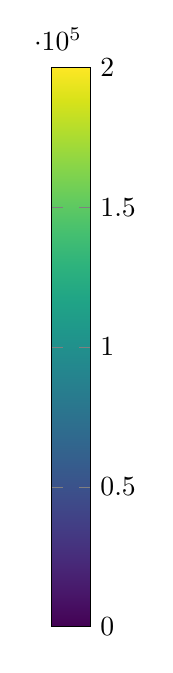
\begin{tikzpicture}
    \begin{axis}[
        hide axis,
        scale only axis,
        height=8.8cm,
        width=0pt,
        point meta min=0,
        point meta max=200000,
        colormap name=viridis,
        colorbar = true,
        colorbar style={
            height=7.1cm,
        }
    ]
    \addplot [draw=none] coordinates {(0,0)};
    \end{axis}
    \end{tikzpicture}
    \end{minipage}

    \caption{Średnia liczba zapytań typu stack content query}
\end{figure}

\FloatBarrier

\begin{figure}[ht]
    \centering

    \begin{minipage}{0.85\textwidth}
        \centering

        \begin{minipage}{0.48\textwidth}
            \centering
            \begin{tikzpicture}
    \begin{axis}[
        baseMetricsHeatmap,
        colorbar = true,
        point meta min=1,
        point meta max=16,
        xlabel={liczba symboli call},
        xmin=3, xmax=15,
        ymin=2, ymax=16,
        xtick={3,5,...,15},
        ytick={2,4,...,16},
    ]
    \addplot [
        matrix plot*,
        point meta=explicit,
        mesh/rows=7,
    ] coordinates {
        (3, 2) [2.745]
        (3, 4) [5.91]
        (3, 6) [8.1]
        (3, 8) [9.625]
        (3, 10) [11.075]
        (3, 12) [11.96]
        (3, 14) [12.82]
        (3, 16) [13.835]

        (5, 2) [2.84]
        (5, 4) [6.055]
        (5, 6) [8.37]
        (5, 8) [9.925]
        (5, 10) [11.295]
        (5, 12) [12.625]
        (5, 14) [13.465]
        (5, 16) [14.115]

        (7, 2) [2.87]
        (7, 4) [6.155]
        (7, 6) [8.25]
        (7, 8) [9.96]
        (7, 10) [11.195]
        (7, 12) [12.605]
        (7, 14) [13.475]
        (7, 16) [14.335]

        (9, 2) [2.855]
        (9, 4) [6.115]
        (9, 6) [8.355]
        (9, 8) [10.225]
        (9, 10) [11.325]
        (9, 12) [12.62]
        (9, 14) [13.585]
        (9, 16) [14.235]

        (11, 2) [2.81]
        (11, 4) [6.22]
        (11, 6) [8.295]
        (11, 8) [10.085]
        (11, 10) [11.435]
        (11, 12) [12.665]
        (11, 14) [13.35]
        (11, 16) [14.465]

        (13, 2) [2.785]
        (13, 4) [6.245]
        (13, 6) [8.21]
        (13, 8) [10.175]
        (13, 10) [11.395]
        (13, 12) [12.605]
        (13, 14) [13.32]
        (13, 16) [14.26]
        
        (15, 2) [2.785]
        (15, 4) [6.21]
        (15, 6) [8.575]
        (15, 8) [10.275]
        (15, 10) [11.22]
        (15, 12) [12.34]
        (15, 14) [13.555]
        (15, 16) [14.39]
    };
    \end{axis}
    \end{tikzpicture}
        \end{minipage}
        \hfill
        \begin{minipage}{0.48\textwidth}
            \centering
            \begin{tikzpicture}
    \begin{axis}[
        baseMetricsHeatmap,
        colorbar = false,
        point meta min=1,
        point meta max=16,
        xlabel={liczba symboli return},
    ]
    \addplot [
        matrix plot*,
        point meta=explicit,
        mesh/rows=7,
    ] coordinates {
        (3, 2) [2.745]
        (3, 4) [5.91]
        (3, 6) [8.1]
        (3, 8) [9.625]
        (3, 10) [11.075]
        (3, 12) [11.96]
        (3, 14) [12.82]
        (3, 16) [13.835]

        (5, 2) [2.93]
        (5, 4) [6.12]
        (5, 6) [8.45]
        (5, 8) [9.95]
        (5, 10) [11.56]
        (5, 12) [12.47]
        (5, 14) [13.315]
        (5, 16) [14.27]

        (7, 2) [3.025]
        (7, 4) [6.44]
        (7, 6) [8.8]
        (7, 8) [10.355]
        (7, 10) [11.665]
        (7, 12) [12.755]
        (7, 14) [13.455]
        (7, 16) [14.18]

        (9, 2) [3.01]
        (9, 4) [6.535]
        (9, 6) [8.76]
        (9, 8) [10.495]
        (9, 10) [11.77]
        (9, 12) [12.865]
        (9, 14) [13.78]
        (9, 16) [14.445]

        (11, 2) [3.06]
        (11, 4) [6.5]
        (11, 6) [8.95]
        (11, 8) [10.785]
        (11, 10) [12.08]
        (11, 12) [13.135]
        (11, 14) [13.925]
        (11, 16) [14.58]

        (13, 2) [3.1]
        (13, 4) [6.54]
        (13, 6) [8.995]
        (13, 8) [10.775]
        (13, 10) [12.335]
        (13, 12) [13.605]
        (13, 14) [14.51]
        (13, 16) [14.98]

        (15, 2) [3.085]
        (15, 4) [6.555]
        (15, 6) [8.95]
        (15, 8) [11.01]
        (15, 10) [12.635]
        (15, 12) [13.58]
        (15, 14) [14.34]
        (15, 16) [15.105]
    };
    \end{axis}
    \end{tikzpicture}
        \end{minipage}

        \vspace{0.5em}

        \begin{minipage}{0.48\textwidth}
            \centering
            \begin{tikzpicture}
    \begin{axis}[
        baseMetricsHeatmap,
        colorbar = false,
        point meta min=1,
        point meta max=16,
        xlabel={liczba symboli local},
    ]
    \addplot [
        matrix plot*,
        point meta=explicit,
        mesh/rows=7,
    ] coordinates {
        (3, 2) [2.745]
        (3, 4) [5.91]
        (3, 6) [8.1]
        (3, 8) [9.625]
        (3, 10) [11.075]
        (3, 12) [11.96]
        (3, 14) [12.82]
        (3, 16) [13.835]

        (5, 2) [2.69]
        (5, 4) [5.945]
        (5, 6) [8.26]
        (5, 8) [9.905]
        (5, 10) [11.215]
        (5, 12) [12.365]
        (5, 14) [13.235]
        (5, 16) [13.92]

        (7, 2) [2.66]
        (7, 4) [5.865]
        (7, 6) [8.14]
        (7, 8) [9.875]
        (7, 10) [11.15]
        (7, 12) [12.32]
        (7, 14) [13.39]
        (7, 16) [14.185]

        (9, 2) [2.725]
        (9, 4) [5.84]
        (9, 6) [7.955]
        (9, 8) [9.75]
        (9, 10) [11.325]
        (9, 12) [12.45]
        (9, 14) [13.43]
        (9, 16) [14.395]

        (11, 2) [2.61]
        (11, 4) [5.725]
        (11, 6) [8.115]
        (11, 8) [9.69]
        (11, 10) [11.165]
        (11, 12) [12.585]
        (11, 14) [13.505]
        (11, 16) [14.275]

        (13, 2) [2.58]
        (13, 4) [5.735]
        (13, 6) [7.905]
        (13, 8) [9.895]
        (13, 10) [11.445]
        (13, 12) [12.685]
        (13, 14) [13.45]
        (13, 16) [14.54]

        (15, 2) [2.605]
        (15, 4) [5.755]
        (15, 6) [8.075]
        (15, 8) [9.875]
        (15, 10) [11.33]
        (15, 12) [12.43]
        (15, 14) [13.745]
        (15, 16) [14.575]
    };
    \end{axis}
    \end{tikzpicture}
        \end{minipage}
        \hfill
        \begin{minipage}{0.48\textwidth}
            \centering
            \begin{tikzpicture}
    \begin{axis}[
        baseMetricsHeatmap,
        colorbar = false,
        point meta min=1,
        point meta max=16,
        xlabel={liczba symboli stosowych},
        xmin=5,
    ]
    \addplot [
        matrix plot*,
        point meta=explicit,
        mesh/rows=6,
    ] coordinates {
        (5, 2) [2.265]
        (5, 4) [4.635]
        (5, 6) [6.73]
        (5, 8) [8.105]
        (5, 10) [9.335]
        (5, 12) [10.42]
        (5, 14) [11.545]
        (5, 16) [12.76]

        (7, 2) [2.35]
        (7, 4) [4.765]
        (7, 6) [6.525]
        (7, 8) [8.16]
        (7, 10) [9.345]
        (7, 12) [10.545]
        (7, 14) [11.505]
        (7, 16) [12.385]

        (9, 2) [2.275]
        (9, 4) [4.665]
        (9, 6) [6.43]
        (9, 8) [8.01]
        (9, 10) [9.065]
        (9, 12) [10.36]
        (9, 14) [11.55]
        (9, 16) [11.935]

        (11, 2) [2.375]
        (11, 4) [4.68]
        (11, 6) [6.415]
        (11, 8) [8.24]
        (11, 10) [9.295]
        (11, 12) [10.29]
        (11, 14) [11.445]
        (11, 16) [12.31]

        (13, 2) [2.295]
        (13, 4) [4.7]
        (13, 6) [6.6]
        (13, 8) [8.035]
        (13, 10) [9.16]
        (13, 12) [10.37]
        (13, 14) [11.435]
        (13, 16) [12.37]

        (15, 2) [2.3]
        (15, 4) [4.815]
        (15, 6) [6.46]
        (15, 8) [7.9]
        (15, 10) [9.48]
        (15, 12) [10.325]
        (15, 14) [11.185]
        (15, 16) [12.485]
    };
    \end{axis}
    \end{tikzpicture}
        \end{minipage}
    \end{minipage}
    \hfill
    \begin{minipage}{0.08\textwidth}
    \centering
    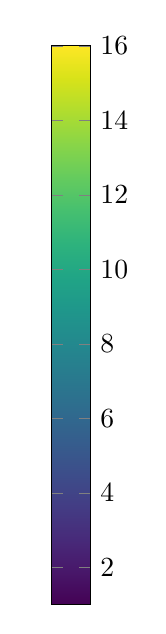
\begin{tikzpicture}
    \begin{axis}[
        hide axis,
        scale only axis,
        height=8.8cm,
        width=0pt,
        point meta min=1,
        point meta max=16,
        colormap name=viridis,
        colorbar = true,
        colorbar style={
            height=7.1cm,
        }
    ]
    \addplot [draw=none] coordinates {(0,0)};
    \end{axis}
    \end{tikzpicture}
    \end{minipage}

    \caption{Średnia liczba zapytań typu equivalence query}
\end{figure}

\FloatBarrier

Podobieństwo wyników przy rosnącej liczbie symboli typu call oraz local jest zaskakujące.
Oczekiwano, że wzrost liczby symboli typu call znacząco zwiększy liczbę zapytań w porównaniu
z symbolami typu local.

\section{Wpływ SRS}

Korzyścią z wykorzystania systemu SRS jest potencjalne zredukowanie liczby zapytań,
skrócenie czasu procesu uczenia oraz poprawa dokładności uczenia w przypadku wykorzystania
heurystycznych podejść do przetwarzania zapytania o równoważność. Dlatego sekcja ta została
podzielona na dwie podsekcje. Pierwsza przedstawia wpływ systemu SRS na wydajność uczenia,
z wykorzystaniem dokładnego algorytmu nauczyciela. Druga wykorzystuje heurystyczne podejście
oraz przedstawia jak system SRS wpływa na dokładność uczenia.

Każdy ze scenariuszy składa się z dwóch iteracji. W pierwszej iteracji system SRS nie jest wykorzystywany.
Przed drugą iteracją ziarno generatora liczb losowych jest ponownie ustawiane w celu wygenerowania
identycznych automatów.

\subsection{Podstawowe metryki}

Sekcja ta przedstawia jak poszczególne typy systemów SRS wpłynęły na proces uczenia pod względem liczby zapytań
equivalence query skierowanych do nauczyciela, oraz czasu działania algorytmu.

Poniżej przedstawiona jest część wspólna początkowej konfiguracji wszystkich
generatorów, które zostały wykorzystane w tej sekcji:
\begin{verbatim}
NumOfCalls = 3
NumOfLocals = 3
NumOfReturns = 3
NumOfStackSymbols = 5
density = 0.8
acceptingStatesDensity = 0.3
\end{verbatim}

Każdy ze scenariuszy modyfikował początkową konfigurację generatora poprzez zwiększanie liczby stanów automatu.
Dla każdej konfiguracji zostało wygenerowane 100 automatów, dla których poszczególne wyniki zostały zebrane i uśrednione.

\paragraph{Cancellation}

\def\DataCexSrs{
    (4, 1.88)
    (6, 2.91)
    (8, 3.95)
    (10, 5.18)
    (12, 6.1)
    (14, 7.06)
    (16, 8.05)
    (18, 8.53)
    (20, 9.55)
    (22, 10.78)
    (24, 11.02)
    (26, 12.53)
    (28, 13.04)
    (30, 14.21)
}

\def\DataEqNoSrs{
    (4, 4.08)
    (6, 6.28)
    (8, 8.17)
    (10, 10.08)
    (12, 11.47)
    (14, 12.68)
    (16, 14.28)
    (18, 15.06)
    (20, 15.81)
    (22, 17.61)
    (24, 18.06)
    (26, 19.48)
    (28, 20.2)
    (30, 20.51)
}

\def\DataEqSrs{
    (4, 2.2)
    (6, 3.37)
    (8, 4.16)
    (10, 5)
    (12, 5.46)
    (14, 5.78)
    (16, 6.53)
    (18, 6.85)
    (20, 6.87)
    (22, 7.23)
    (24, 6.98)
    (26, 7.75)
    (28, 8.33)
    (30, 8.02)
}

\def\DataTimeNoSrs{
    (4, 0.91694)
    (6, 1.42234)
    (8, 1.87105)
    (10, 2.35555)
    (12, 2.77282)
    (14, 3.25221)
    (16, 3.89834)
    (18, 4.4683)
    (20, 5.38287)
    (22, 6.91603)
    (24, 8.40194)
    (26, 11.4513)
    (28, 14.0205)
    (30, 17.2291)
}

\def\DataTimeSrs{
    (4, 1.41132)
    (6, 2.1872)
    (8, 2.82718)
    (10, 3.52833)
    (12, 4.08224)
    (14, 4.64853)
    (16, 5.53962)
    (18, 6.31531)
    (20, 7.33319)
    (22, 8.95478)
    (24, 10.0128)
    (26, 13.3601)
    (28, 15.8366)
    (30, 19.3584)
}





\begin{figure}[H]
\centering
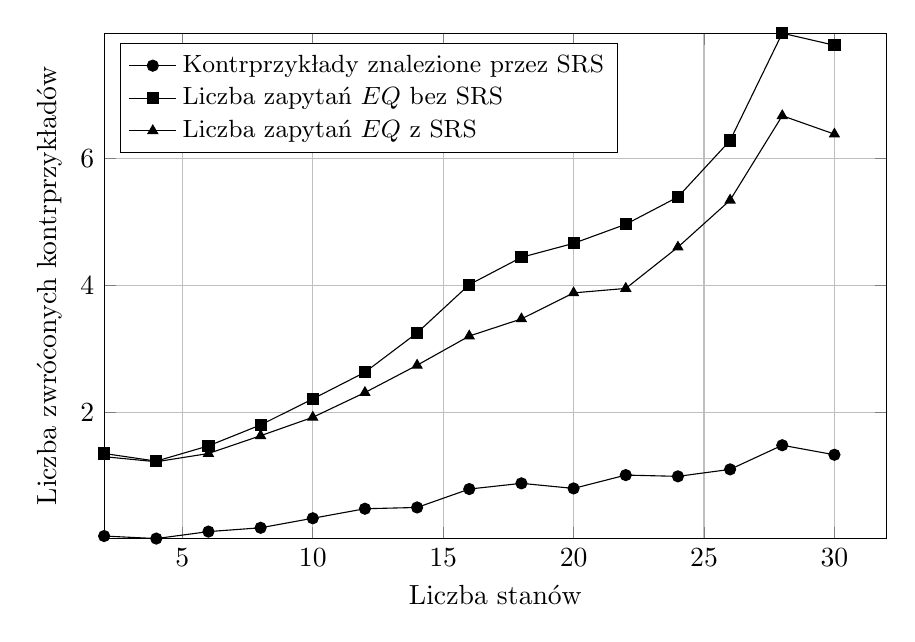
\begin{tikzpicture}
\begin{axis}[
    width=0.95\linewidth,
    height=8cm,
    xlabel={Liczba stanów},
    ylabel={Liczba zwróconych kontrprzykładów},
    grid=major,
    legend style={at={(0.02,0.98)}, anchor=north west, font=\small},
    legend cell align=left,
    xmin=2, xmax=32,
    enlargelimits=false
]
    \addplot[mark=*] coordinates { \DataCexSrs };
    \addlegendentry{Kontrprzykłady znalezione przez SRS}

    \addplot[mark=square*] coordinates { \DataEqNoSrs };
    \addlegendentry{Liczba zapytań $EQ$ bez SRS}

    \addplot[mark=triangle*] coordinates { \DataEqSrs };
    \addlegendentry{Liczba zapytań $EQ$ z SRS}
\end{axis}
\end{tikzpicture}
\caption{Porównanie liczby zapytań o równoważność z użyciem reguł SRS cancellation}
\label{fig:cancellationEq}
\end{figure}

\begin{figure}[H]
\centering
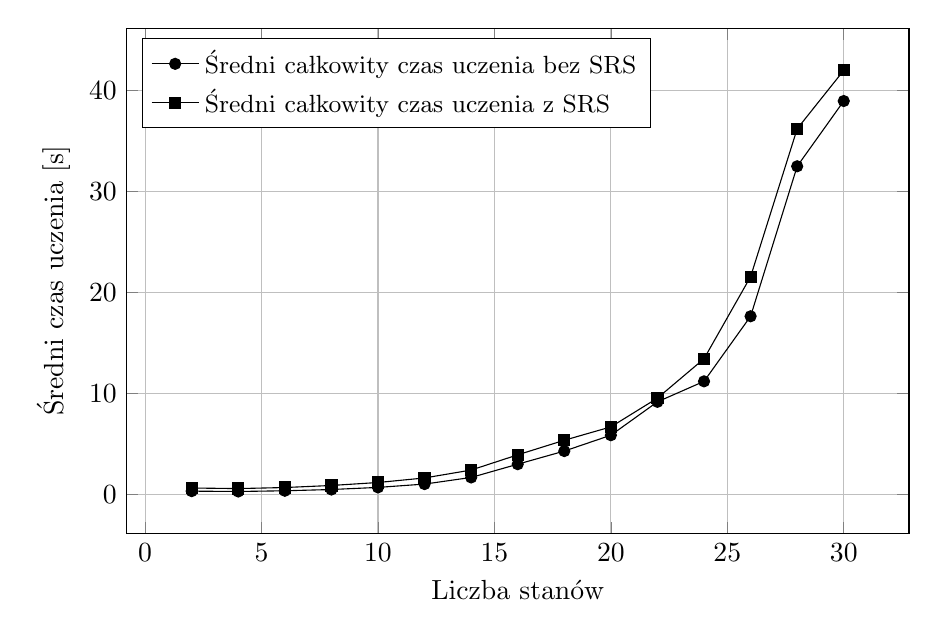
\begin{tikzpicture}
\begin{axis}[
    width=0.95\linewidth,
    height=8cm,
    xlabel={Liczba stanów},
    ylabel={Średni czas uczenia [s]},
    grid=major,
    legend style={at={(0.02,0.98)}, anchor=north west, font=\small},
    legend cell align=left
]
    \addplot[mark=*] coordinates { \DataTimeNoSrs };
    \addlegendentry{Średni całkowity czas uczenia bez SRS}

    \addplot[mark=square*] coordinates { \DataTimeSrs };
    \addlegendentry{Średni całkowity czas uczenia z SRS}
\end{axis}
\end{tikzpicture}
\caption{Porównanie całkowitego czasu uczenia, obejmującego czas działania ucznia i nauczyciela, z użyciem reguł SRS cancellation}
\label{fig:cancellationTime}
\end{figure}


Z każdym wygenerowanym automatem była związana następująca reguła SRS $cXr \rightarrow \epsilon$.
Jednak na podstawie obserwacji i przeprowadzonych testów okazuje się, że dla wygenerowanych automatów
równie skuteczna jest reguła $cr \rightarrow \epsilon$. Obserwacja ta jednak nie przełożyła się na skuteczność
uczenia opisaną w następnej sekcji.

\paragraph{Commutation}

\def\DataCexSrs{
    (4, 0.84)
    (6, 0.97)
    (9, 1.19)
    (12, 1.23)
    (15, 1.79)
    (16, 1.41)
    (18, 1.88)
    (20, 1.77)
    (25, 2.21)
    (30, 2.5)
}

\def\DataEqNoSrs{
    (4, 2.56)
    (6, 3.68)
    (9, 4.28)
    (12, 5.44)
    (15, 6.99)
    (16, 5.96)
    (18, 7.72)
    (20, 7.33)
    (25, 9.03)
    (30, 10.55)
}

\def\DataEqSrs{
    (4, 1.37)
    (6, 2.27)
    (9, 3.2)
    (12, 4.02)
    (15, 5.47)
    (16, 5.17)
    (18, 5.97)
    (20, 5.91)
    (25, 6.96)
    (30, 8.52)
}

\def\DataTimeNoSrs{
    (4, 0.689737)
    (6, 1.25931)
    (9, 2.4844)
    (12, 6.01334)
    (15, 15.0101)
    (16, 12.3133)
    (18, 34.5499)
    (20, 29.7876)
    (25, 82.7877)
    (30, 249.934)
}

\def\DataTimeSrs{
    (4, 0.948409)
    (6, 1.78883)
    (9, 3.89908)
    (12, 9.48304)
    (15, 26.5288)
    (16, 18.5707)
    (18, 43.2236)
    (20, 42.619)
    (25, 101.328)
    (30, 220.468)
}





\begin{figure}[H]
\centering
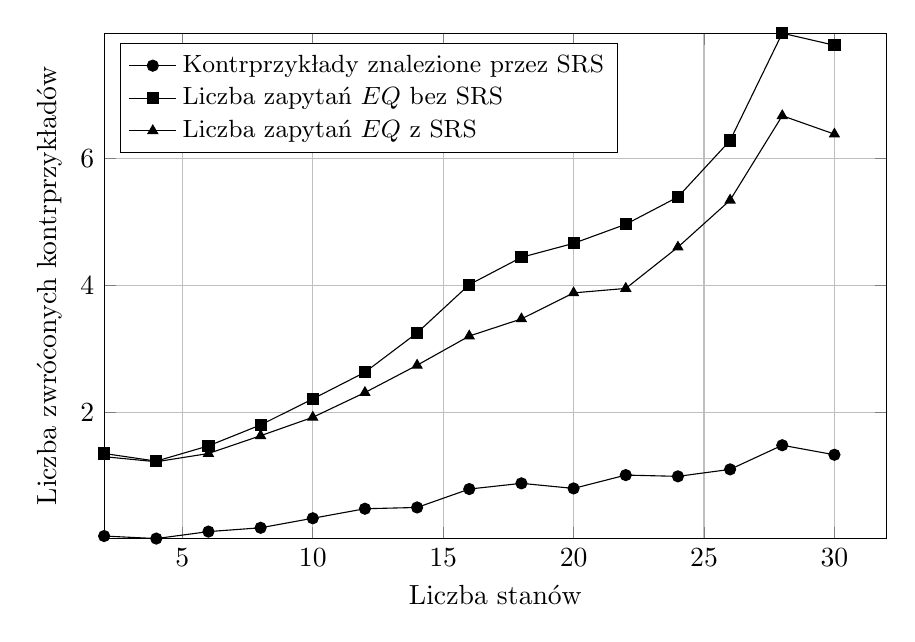
\begin{tikzpicture}
\begin{axis}[
    width=0.95\linewidth,
    height=8cm,
    xlabel={Liczba stanów},
    ylabel={Liczba zwróconych kontrprzykładów},
    grid=major,
    legend style={at={(0.02,0.98)}, anchor=north west, font=\small},
    legend cell align=left,
    xmin=2, xmax=32,
    enlargelimits=false
]
    \addplot[mark=*] coordinates { \DataCexSrs };
    \addlegendentry{Kontrprzykłady znalezione przez SRS}

    \addplot[mark=square*] coordinates { \DataEqNoSrs };
    \addlegendentry{Liczba zapytań $EQ$ bez SRS}

    \addplot[mark=triangle*] coordinates { \DataEqSrs };
    \addlegendentry{Liczba zapytań $EQ$ z SRS}
\end{axis}
\end{tikzpicture}
\caption{Porównanie liczby zapytań o równoważność z użyciem reguł SRS commutation}
\label{fig:commutationEq}
\end{figure}

\begin{figure}[H]
\centering
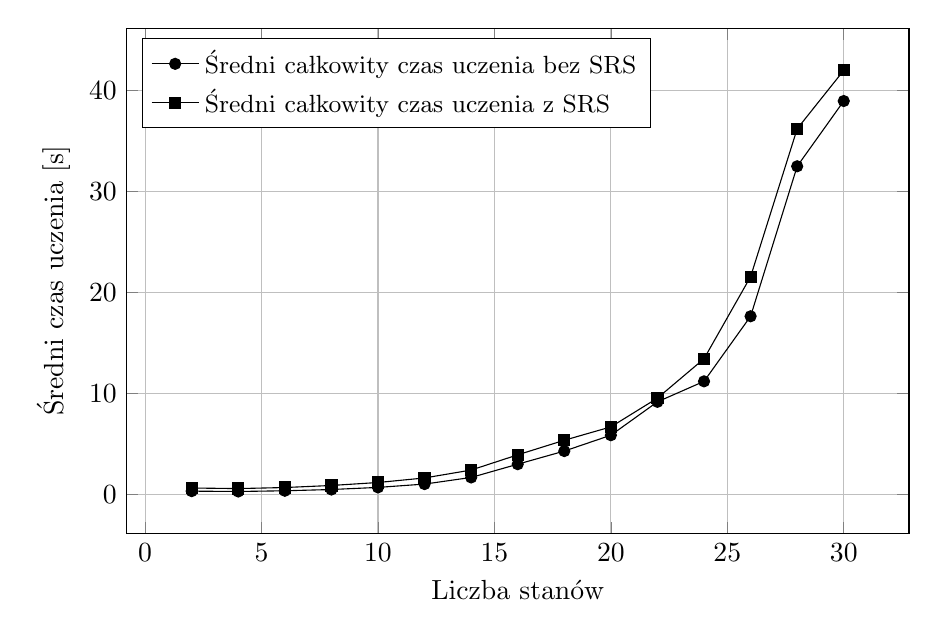
\begin{tikzpicture}
\begin{axis}[
    width=0.95\linewidth,
    height=8cm,
    xlabel={Liczba stanów},
    ylabel={Średni czas uczenia [s]},
    grid=major,
    legend style={at={(0.02,0.98)}, anchor=north west, font=\small},
    legend cell align=left
]
    \addplot[mark=*] coordinates { \DataTimeNoSrs };
    \addlegendentry{Średni całkowity czas uczenia bez SRS}

    \addplot[mark=square*] coordinates { \DataTimeSrs };
    \addlegendentry{Średni całkowity czas uczenia z SRS}
\end{axis}
\end{tikzpicture}
\caption{Porównanie całkowitego czasu uczenia, obejmującego czas działania ucznia i nauczyciela, z użyciem reguł SRS commutation}
\label{fig:commutationTime}
\end{figure}


Wyniki dla tej reguły nie są zadowalające, bazując na analogicznych wynikach dla automatów DFA~\cite{srs}
spodziewana była znacznie większa redukcja liczby zapytań, co również przełożyłoby się na czas uczenia.
Możliwe jest, że sposób generowania automatów dla tej reguły nie pozwolił ukazać jej całkowitego potencjału.

\paragraph{Idempotency}

\def\DataCexSrs{
    (2, 0.05)
    (4, 0.01)
    (6, 0.12)
    (8, 0.18)
    (10, 0.33)
    (12, 0.48)
    (14, 0.5)
    (16, 0.79)
    (18, 0.88)
    (20, 0.8)
    (22, 1.01)
    (24, 0.99)
    (26, 1.1)
    (28, 1.48)
    (30, 1.33)
}

\def\DataEqNoSrs{
    (2, 1.35)
    (4, 1.23)
    (6, 1.47)
    (8, 1.8)
    (10, 2.21)
    (12, 2.63)
    (14, 3.25)
    (16, 4.01)
    (18, 4.44)
    (20, 4.66)
    (22, 4.96)
    (24, 5.39)
    (26, 6.28)
    (28, 7.97)
    (30, 7.78)
}

\def\DataEqSrs{
    (2, 1.3)
    (4, 1.22)
    (6, 1.35)
    (8, 1.63)
    (10, 1.92)
    (12, 2.31)
    (14, 2.74)
    (16, 3.2)
    (18, 3.47)
    (20, 3.88)
    (22, 3.95)
    (24, 4.6)
    (26, 5.34)
    (28, 6.67)
    (30, 6.38)
}

\def\DataTimeNoSrs{
    (2, 0.335162)
    (4, 0.300043)
    (6, 0.371178)
    (8, 0.495983)
    (10, 0.705462)
    (12, 1.03486)
    (14, 1.69011)
    (16, 3.00451)
    (18, 4.30489)
    (20, 5.87462)
    (22, 9.18305)
    (24, 11.2126)
    (26, 17.6587)
    (28, 32.5181)
    (30, 38.9832)
}

\def\DataTimeSrs{
    (2, 0.644327)
    (4, 0.588754)
    (6, 0.692957)
    (8, 0.896431)
    (10, 1.18994)
    (12, 1.64141)
    (14, 2.42388)
    (16, 3.93291)
    (18, 5.37635)
    (20, 6.70033)
    (22, 9.55163)
    (24, 13.4512)
    (26, 21.5843)
    (28, 36.2319)
    (30, 42.0227)
}





\begin{figure}[H]
\centering
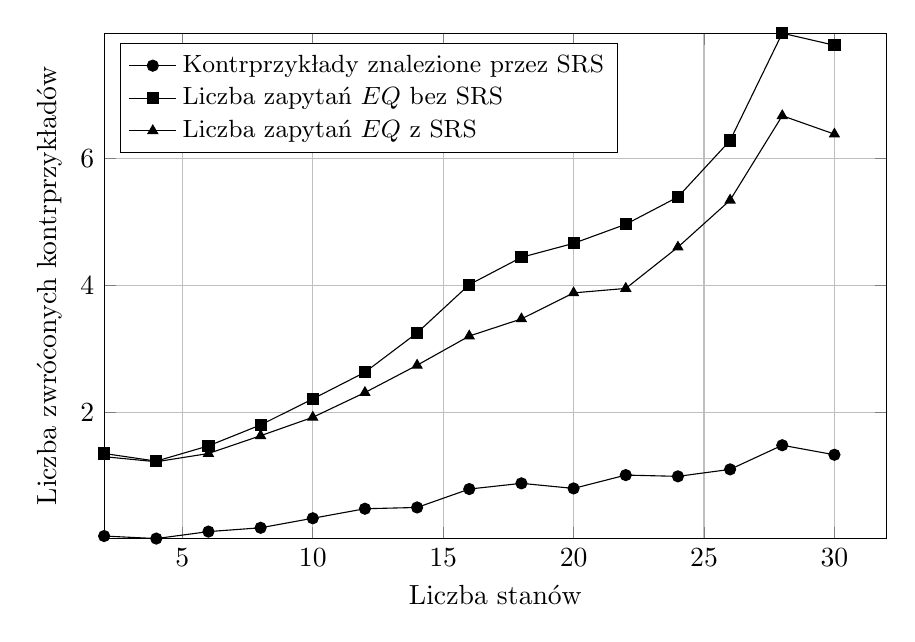
\begin{tikzpicture}
\begin{axis}[
    width=0.95\linewidth,
    height=8cm,
    xlabel={Liczba stanów},
    ylabel={Liczba zwróconych kontrprzykładów},
    grid=major,
    legend style={at={(0.02,0.98)}, anchor=north west, font=\small},
    legend cell align=left,
    xmin=2, xmax=32,
    enlargelimits=false
]
    \addplot[mark=*] coordinates { \DataCexSrs };
    \addlegendentry{Kontrprzykłady znalezione przez SRS}

    \addplot[mark=square*] coordinates { \DataEqNoSrs };
    \addlegendentry{Liczba zapytań $EQ$ bez SRS}

    \addplot[mark=triangle*] coordinates { \DataEqSrs };
    \addlegendentry{Liczba zapytań $EQ$ z SRS}
\end{axis}
\end{tikzpicture}
\caption{Porównanie liczby zapytań o równoważność z użyciem reguł SRS idempotency}
\label{fig:idempotencyEq}
\end{figure}

\begin{figure}[H]
\centering
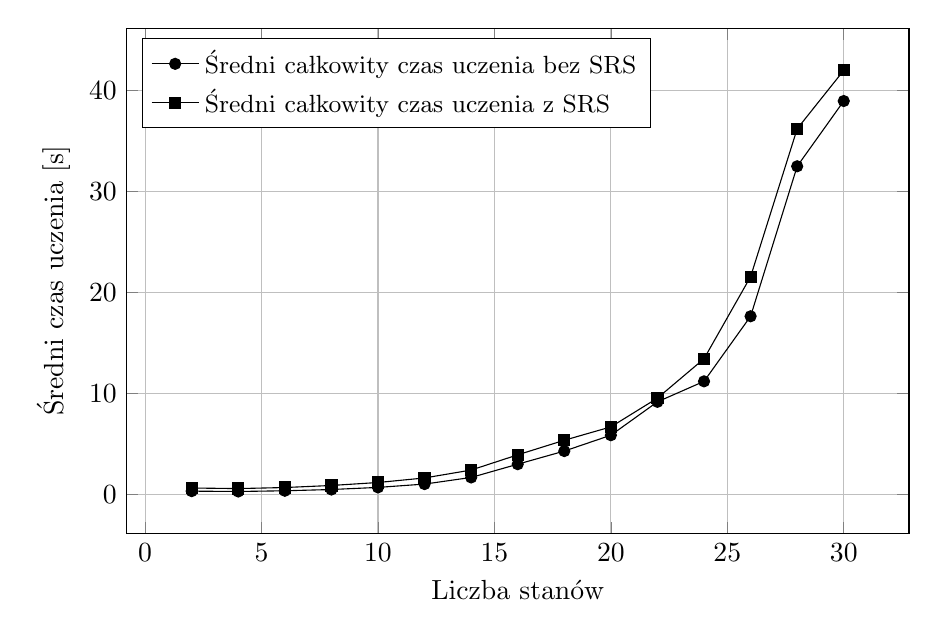
\begin{tikzpicture}
\begin{axis}[
    width=0.95\linewidth,
    height=8cm,
    xlabel={Liczba stanów},
    ylabel={Średni czas uczenia [s]},
    grid=major,
    legend style={at={(0.02,0.98)}, anchor=north west, font=\small},
    legend cell align=left
]
    \addplot[mark=*] coordinates { \DataTimeNoSrs };
    \addlegendentry{Średni całkowity czas uczenia bez SRS}

    \addplot[mark=square*] coordinates { \DataTimeSrs };
    \addlegendentry{Średni całkowity czas uczenia z SRS}
\end{axis}
\end{tikzpicture}
\caption{Porównanie całkowitego czasu uczenia, obejmującego czas działania ucznia i nauczyciela, z użyciem reguł SRS idempotency}
\label{fig:idempotencyTime}
\end{figure}


Odpowiadająca tej regule reguła dla automatów DFA w postaci $uu \rightarrow u$ w pracy~\cite{srs}
została przedstawiona, jako przynosząca najmniejsze korzyści. Jednak nie było oczywiste, że obserwacja
ta powtórzy się dla automatów DVPA z powodu zastosowania reguł z parametrem.
Jednakże, otrzymane wyniki potwierdzają tę obserwację również dla automatów DVPA.

\paragraph{Podsumowanie}
W przeprowadzonych eksperymentach wykorzystanie systemu SRS prowadziło do redukcji liczby zapytań o równoważność.
W przypadku reguł typu cancellation redukcja ta wyniosła około $50\%$, natomiast w przypadku commutation i
idempotency około $20\%$.

Czas uczenia w większości przypadków zwiększył się, jednak widoczna jest tendencja zmniejszania narzutu czasowego dla większych automatów.
Może to sugerować, że dla większych instancji wykorzystanie systemu SRS będzie bardziej opłacalne czasowo.


\subsection{Wpływ SRS na dokładność uczenia}

W celu heurystycznego sprawdzenia równoważności dwóch automatów dla każdego zapytania wygenerowano
$N$ losowych słów o losowej długości ograniczonej do 100 liter. Ta sama heurystyka była wykorzystywana podczas
sprawdzania spójności hipotezy z systemem SRS. Ostateczna ocena, czy zwrócony przez algorytm automat jest
zgodny z automatem docelowym odbywała się poprzez dokładne sprawdzenie wykorzystywane w algorytmie nauczyciela.

Ponieważ wykorzystanie systemu SRS powodowało, że w trakcie uczenia wykonywane były dodatkowe heurystyczne
sprawdzenia równoważności, wariant bez systemu SRS został przetestowany dla $N = 10^5$ oraz $N = 2 \cdot 10^5$.
Pozwala to porównać wpływ systemu SRS z prostym zwiększeniem liczby losowo generowanych słów.
Dla każdej reguły wygenerowano $10^4$ losowych automatów, które zawierały od $10$ do $25$ stanów.

\begin{table}[H]
\centering
\begin{tabular}{cc|ccc}
\hline
Reguła SRS & Metryka
& $N = 10^5$
& $N = 2\cdot10^5$
& $N = 10^5$ z SRS \\
\hline
\multirow{2}{*}{Cancellation}
& Odsetek sukcesów & 30.29\% & 40.1\% & 57.19\% \\
& Średni czas [s] & 0.69 & 1.28 & 2.6 \\
\hline
\multirow{2}{*}{Commutativity}
& Odsetek sukcesów & 73.93\% & 78.59\% & 74.11\% \\
& Średni czas [s] & 0.69 & 0.89 & 2.0 \\
\hline
\multirow{2}{*}{Idempotency}
& Odsetek sukcesów & 91.0\% & 93.24\% & 91.69\% \\
& Średni czas [s] & 0.38 & 0.78 & 0.92 \\
\hline
\end{tabular}
\caption{Porównanie skuteczności oraz średniego czasu uczenia}
\end{table}

Zwiększony czas wykonania wynika głównie z zastosowanej heurystyki do wyboru słów dobrze zbalansowanych.
Jednak całkowity czas uczenia z wykorzystaniem tego podejścia jest znacząco mniejszy niż w przypadku
dokładnego sprawdzenia, gdzie narzut wykorzystanej heurystyki jest pomijalnie mały. Oznacza to, że pomimo zwiększonego
średniego czasu uczenia jednego automatu narzut ten nie powinien stanowić problemu w praktycznym wykorzystaniu.

Zwiększenie skuteczności podejścia heurystycznego jest szczególnie widoczne w przypadku reguły Cancellation,
wyniki dla dwóch pozostałych reguł nie wskazują znaczącej poprawy. Jednakże wykorzystanie tej funkcjonalności może
poprawiać skuteczność, co czyni je wartościową funkcjonalnością w przypadku użycia heurystycznego sprawdzania
równoważności.